\chapter{Dasar Python}

\section{Tipe Data Python}

Dalam konteks tipe data python memiliki sifat sebagai berikut.
\begin{enumerate}
	\item \textit{Dynamically Typed}: python akan menentukan secara sendiri tipe data dari setiap variabel yang kita gunakan tanpa harus perlu deklarasi di awal.
	\item \textit{Strongly Typed} yang berarti operasi tertentu hanya bisa dilakukan berdasarkan tipe data yang benar. 
\end{enumerate}

Walaupun python tidak memerlukan secara eksplisit menuliskan tipe data ketika mendeklarasikan variabel, semua variabel yang dideklarasikan tetap termasuk ke dalam tipe data built-in python. Tipe data python bisa dilihat di Table \ref{tbl:tipeDataPython}.

\begin{table}[H]%
\caption{Tipe data built-in}
\centering
\begin{tabular}{|l|l|}
\hline
Tipe Objek & Contoh \\
\hline
Numbers & 111234, 3.1415, 999L, 3+4j, Decimal\\
Strings & 'spam', "guido's"\\
Lists & [1, [2, 'three'], 4]\\
Dictionaries & {'food': 'spam', 'taste': 'yum'}\\
Tuples & (1,'spam', 4, 'U')\\
Files & myfile = open('eggs', 'r')\\
Other types & Sets, types, None, Booleans\\
\hline
\end{tabular}
\label{tbl:tipeDataPython}
\end{table} 

\section{Pengenalan IDLE dan IDE (PyScripter)}

\subsection{IDLE}

\begin{panduan}{Dasar variabel}
\begin{enumerate}
	\item Buka IDLE seperti di bawah ini:
	\begin{figure}[H]%
		\centering
		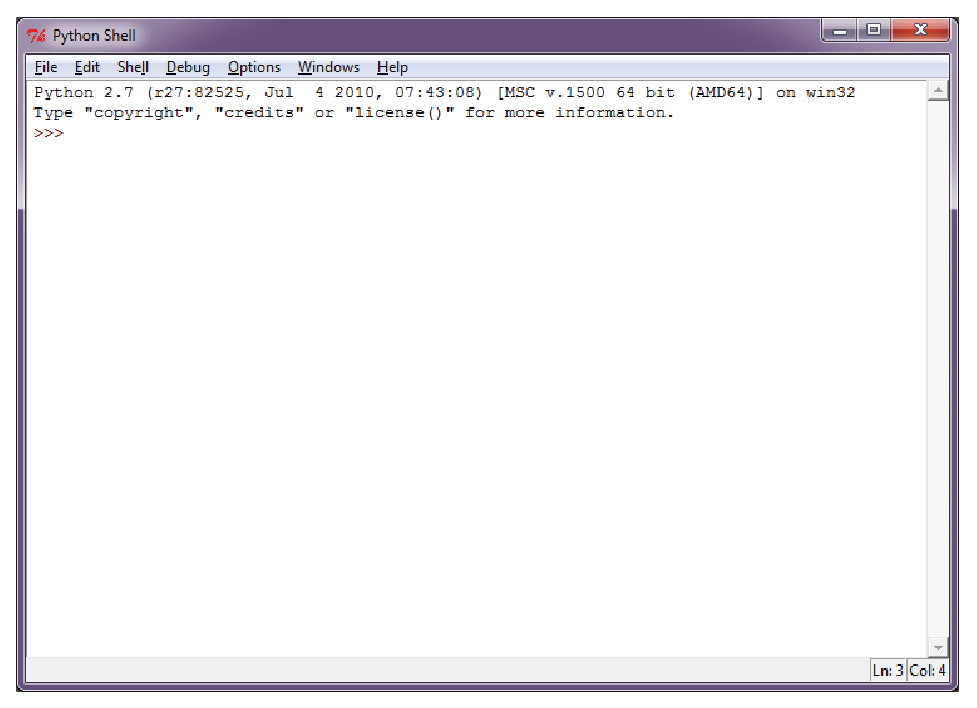
\includegraphics[scale=0.6]{fig/IDLE.eps}%
	\end{figure}
	\item Sebagai pengantar, ketikkan: 
	\begin{IDLE}
		\begin{tabbing}
		$>>>$ a = 4\\
		$>>>$ a ~~~~~~~~~~~~~~~~~~~~~~~~~~~~~~~~~~~~ \= \# \textit{Menampilkan hasil dari `a'}\\
		\textbf{4}\\
		$>>>$ a + 4\\
		\textbf{8}\\
		$>>>$ a\\
		\textbf{4}\\
		$>>>$ a = a + 4\\
		$>>>$ a\\
		\textbf{8}\\
		$>>>$ a + 1, a - 1\> \# \textit{Dua perintah dalam satu baris sekaligus}\\
		\textbf{9,7}\\
		$>>>$ a * 3, a / 2 \> \# \textit{Mengalikan dan membagi nilai `a'}\\
		\textbf{24,4}\\
		$>>>$ a \% 3, a ** 2 \> \# \textit{Modulo dan eksponen nilai `a'}\\
		\textbf{2,64}\\
		$>>>$ import math \> \# \textit{Import modul math}\\
		$>>>$ math.pi \> \# \textit{Menampilkan nilai pi (tidak semuanya)}\\
		\textbf{3.1415926535897931}\\
		$>>>$ math.sqrt(85) \> \# \textit{Akar dari nilai 85}\\
		\textbf{9.2195444572928871} \\
		$>>>$ import random \> \# \textit{Import modul random}\\
		$>>>$ random.random() \> \# \textit{Menampilkan bilangan acak 0 ~ 1}\\
		\textbf{0.3990536432569244}\\
		$>>>$ random.choice([23,54,13,44]) \> \# \textit{Memilih salah satu bilangan}\\
		\textbf{23}\\
		\end{tabbing}
	\end{IDLE}
\end{enumerate}
\end{panduan}

\begin{latihan}
Hitunglah dengan menggunakan python langkah-langkah berikut:
\begin{enumerate}
	\item Isi $a$ dengan 300
	\item Isi $b$ dengan 700
	\item Kalikan $a$ dengan $b$ dan taruh di dalam $c$
	\item Isi $d$ dengan 1200
	\item Tambahkan isi $a$ dengan 60 dan kemudian kalikan hasil tersebut dengan $10$ dan simpan kembali ke $a$   
	\item Bagikan $a$ dengan $d$ dan isi ke dalam $e$
	\item Tambahkan $b$ dengan $c$ dan isi ke dalam $c$
	\item Tambahkan $a$ dengan $e$ kemudian kurangkan dengan $c$ dan simpan ke $b$
\end{enumerate}
Berapakah hasil akhir variabel $a$, $b$, $c$, $d$, dan $e$? 
Tuliskan langkah-langkah yang anda ketikkan di secarik kertas.
\end{latihan}

\begin{latihan}
Ada lima variabel yaitu $a$ = 1, $b$ = 2, $c$ = 3, $d$ = 4, dan $e$ = 5. Tukarkan variabel tersebut sehingga hasilnya $a$ = 5, $b$ = 3, $c$ = 4, $d$ = 1, $e$ = 2. Tuliskan langkah-langkah yang anda ketikkan di secarik kertas. 
\end{latihan}

\begin{panduan}{Bilangan desimal}
\begin{enumerate}
	\item Buka IDLE
	\item Ketikkan:
	\begin{IDLE}
		\begin{tabbing}
			$>>>$ a = 9/2~~~~~~~~~~~~~~~~~~~~~~~~~~~~~~~~~ \= \# \textit{Melakukan pembagian}\\
			$>>>$ a \\
			4 \> \# \textit{Hasilnya merupakan bulat. Kenapa?}\\
			$>>>$  a = 9.0/2 \\
			$>>>$ a \\
			4.5 \> \# \textit{Sekarang hasilnya desimal. Kenapa?}\\
			$>>>$ a = 9/2.0 \\
			$>>>$ a \\
			4.5 \> \# \textit{Sama, hasilnya desimal. Kenapa?}\\
			$>>>$ a = float(9)/2 \> \# \textit{Melakukan casting ke float(desimal)}\\
			$>>>$ a \\
			4.5 \\
			$>>>$ b = int(a) \> \# \textit{Mengubah float(desimal) menjadi int(bulat)}\\
			$>>>$ b \\
			4\\ 
		\end{tabbing}
	\end{IDLE}
\end{enumerate}
\end{panduan}

\begin{panduan}{String}
\begin{enumerate}
	\item Buka IDLE
	\item Ketikkan:
	\begin{IDLE}
		\begin{tabbing}
		$>>>$ S = 'Spam' \\
		$>>>$ S ~~~~~~~~~~~~~~~~~~~~~~~~~~~~~~~~~~~~ \= \# \textit{Menampilkan hasil dari `S'}\\
		\textbf{'Spam'}\\
		$>>>$ len(S) \> \# \textit{Panjang dari `S'}\\
		\textbf{4}\\
		$>>>$ S[0] \> \# \textit{Karakter pertama dari `S'}\\
		\textbf{'S'}\\
		$>>>$ S[-1] \> \# \textit{Karakter terakhir dari `S'}\\
		\textbf{'m'}\\
		$>>>$ S[1:3] \> \# \textit{Irisan S dari karakter 2 sampai 4}\\
		\textbf{'pa'}\\
		$>>>$ S[1:] \> \# \textit{Irisan S dari karakter 1 sampai habis}\\
		\textbf{'pam'}\\
		$>>>$ S[:3] \> \# \textit{Irisan S dari awal sampai karakter 3}\\
		\textbf{'Spa'}\\
		$>>>$ S[:-1] \> \# \textit{Irisan S dari awal sampai karakter 1 dari belakang}\\
		\textbf{'Spa'}\\
		$>>>$ S[:] \> \# \textit{Semua isi dari S}\\
		\textbf{'Spam'}\\
		$>>>$ S + 'xyz' \> \# \textit{Penambahan karakter tetapi tidak disimpan ke `S'}\\
		\textbf{'Spamxyz}\\
		$>>>$ S * 8 \> \# \textit{Repetisi}\\
		\textbf{'SpamSpamSpamSpamSpamSpamSpamSpam'}
		\end{tabbing}
	\end{IDLE}	
\end{enumerate}
\end{panduan}

\begin{panduan}{List}
\begin{enumerate}
	\item Buka IDLE.
	\item Ketikkan:
		\begin{IDLE}
		\begin{tabbing}
		$>>>$ L = [123, 'spam', 1.23] ~~~~~~~~~~~~~~~~~~~~~ \= \\
		$>>>$ len(L) \> \# \textit{Menampilkan jumlah elemen dari `L'}\\
		\textbf{3}\\
		$>>>$ L[0]\\
		\textbf{123}\\
		$>>>$ L[:-1]\\
		\textbf{[123, 'spam']}\\
		$>>>$ L + [4,5,6]\\
		\textbf{[123, 'spam', 1.23, 4, 5, 6]}\\
		$>>>$ L.append('NI') \> \# \textit{Menambah elemen 'NI' ke `L'}\\
		$>>>$ L \\
		\textbf{[123, 'spam', 1.23, 'NI']} \\
		$>>>$ L.pop(2) \> \# \textit{Membuang elemen ketiga teratas}\\
		\textbf{1.23} \\
		$>>>$ L \\ 
		\textbf{[123, 'spam', 'NI']} \\
		$>>>$ M = [[1,2,3],[4,5,6],[7,8,9]] \> \# \textit{Matriks 3x3}
		\end{tabbing}
		\end{IDLE}	
\end{enumerate}
\end{panduan}

\begin{panduan}{Dictionaries}
\begin{enumerate}
	\item Buka IDLE.
	\item Ketikkan:
		\begin{IDLE}
		\begin{tabbing}
		$>>>$ D = {'food':'Spam', 'quantity':4, 'color':'pink'} \\
		$>>>$ D['food'] ~~~~~~~~~~~~~~~~~~~~~~~~~~~~~~~~~~~~~~~~~ \=  \# \textit{Mengambil data}
		\textbf{'Spam'} \\
		$>>>$ D['quantity'] += 1 \\
		$>>>$ D \\ 
		\textbf{\{'food': 'Spam', 'color':'pink', 'quantity':5\}} \\
		$>>>$ D = \{\} \\
		$>>>$ D \\
		\textbf{\{\}}\\
		$>>>$ D['nama'] = 'Bob' \\
		$>>>$ D['pekerjaan'] = 'programmer' \\
		$>>>$ D['umur'] = 40 \\
		$>>>$ D \\
		\textbf{\{'umur': 40, 'pekerjaan':'programmer', 'nama':'Bob'\}}
		\end{tabbing}
		\end{IDLE}	
\end{enumerate}
\end{panduan}

\subsection{IDE}

Untuk input dari keyboard, python menggunakan sintaks seperti di Listing \ref{lst:inputPython}
\begin{listprog}{Input di Python (input.py)}
	\label{lst:inputPython}
	\begin{lstlisting}[language=Python]
	umur = input("Berapa umur anda?")
	print "Umur anda adalah: ", umur, "tahun."
	\end{lstlisting}
\end{listprog}
\begin{panduan}{Input}
\begin{enumerate}
	\item Buka \textbf{PyScripter for Python 2.7}
	\item Ketikkan Listing \ref{lst:inputPython}.
	\item Tekan CTRL-F9 untuk jalankan.
	\item Save sebagai input.py
\end{enumerate}
\end{panduan}

\begin{latihan}
Buatkan program yang meminta input untuk NIM, nama, jenis kelamin, dan umur anda. Kemudian tampilkan informasi berikut dengan sintaks print.
\end{latihan}

\begin{latihan}
Buatkan program yang bisa menghitung luas segitiga, luas segiempat dan luas lingkaran. Tentukan variabel apa yang perlu diinput dan tampilkan informasi luas dengan menggunakan sintaks print.
\end{latihan}
